\DontFrameThisInToc
\Annex{Annexe sur les assistants conversationnels (\textit{chatbots})}
\label{annex:B-ANNEXE-CHATBOTS}
	
	% INTRODUCTION DE L'ANNEXE.
	
	% Engoument pour les chatbots en 2019.
	Au début de ce doctorat (\texttt{octobre 2019}), nous pouvions noter que :
	\begin{itemize}
		\item selon \cite{costello-lodolce:2019:gartner-top-technologies}, \textguillemets{\textit{seuls $4$\% des clients de \texttt{Gartner} [déclaraient] utiliser des \textit{chatbots} sur leur lieu de travail, mais $40$\%} [avaient] \textit{l'intention de les mettre en oeuvre à court terme}} ;
		\item et selon \cite{goasduff:2019:chatbots-will-appeal}, \textguillemets{\textit{d'ici 2022, 70\% des employés} [interagiraient] \textit{quotidiennement avec les plateformes conversationnelles}}.
	\end{itemize}
	
	% Engoument pour les chatbots en 2023.
	Aujourd'hui (\texttt{octobre 2023}), le mot \textit{chatbot} est présent sur toutes les lèvres, surtout depuis la révolution des \texttt{IA} génératives lancées par \texttt{ChatGPT} (\cite{openai:2023:chatgpt}) :
	\begin{itemize}
		\item selon \cite{costello-lodolce:2022:gartner-predicts-chatbots}, une entreprise sur deux aurait actuellement recours à une forme de \textit{chatbot} pour gérer sa relation client, et \textguillemets{\textit{d'ici 2027, les \textit{chatbots} deviendront le principal canal de service client pour environ un quart des organisations}}.
	\end{itemize}

	% Annonce du plan.
	Dans cette annexe, nous allons détailler les points suivants :
	\begin{itemize}
		\item une présentation rapide de ce qu'est un assistant conversationnel et de ses principales utilisations (voir \textsc{Section~\ref{annex:B.1-ANNEXE-CHATBOTS-PRESENTATION}}) ;
		\item une description des approches principales permettent de concevoir un assistant conversationnel, avec leurs avantages et leurs inconvénients (voir \textsc{Section~\ref{annex:B.2-ANNEXE-CHATBOTS-APPROCHES}}) ;
		\item une discussion sur le dilemme des choix de conception (voir \textsc{Section~\ref{annex:B.3-ANNEXE-CHATBOTS-DILEMME}}).
	\end{itemize}
	
	% TABLE DES MATIÈRES DE L'ANNEXE.
	\minitoc
	
	% \texttt{ChatGPT} (\cite{openai:2023:chatgpt}) et \texttt{BARD} (\cite{google:2023:bard-chat-based}) pour discuter avec des larges modèles de langues (\texttt{LLM}).

	%%%%%--------------------------------------------------------------------
	%%%%% Annexe B.1: Présentation rapide des assistants conversationnels
	%%%%%--------------------------------------------------------------------
	\newpage
	\section{Présentation rapide des assistants conversationnels}
	\label{annex:B.1-ANNEXE-CHATBOTS-PRESENTATION}
	
		%%% Fonctionnalités.
		Les \textit{chatbots} sont des robots conversationnels permettant à un utilisateur d'obtenir des informations ou d'automatiser des actions à l'aide d'instructions en langage naturel.
		\begin{itemize}
			\item[\faThumbsUp] L'utilisation de tels assistants comporte \textbf{plusieurs avantages} :
			ces derniers permettent de réduire les coûts en d'automatisant des tâches simples et répétitives (\textit{permettant aux ainsi aux humaines de se concentrer sur les autres tâches à risques ou à forte valeur ajoutée}),
			ils sont réactifs et toujours accessibles (\textit{au milieu de la nuit, les jours fériés, et même après 16h un vendredi après}),
			et ils ont un comportement stable quelle que soit la situation (\textit{pas de sauts d'humeur, de fatigue ou d'erreurs d'inattention}).
			\item[\faThumbsDown] Néanmoins, ces assistants rencontrent aussi \textbf{plusieurs inconvénients} :
			leur compréhension limitée du langage peut introduire des erreurs (\textit{lorsque le sujet est complexe, quand il y a trop ou trop peu de contexte}),
			ils manquent parfois de flexibilité ou d'empathie (\textit{nécessitant alors d'escalader la requête vers un opérateur humain}),
			et les tâches de conception ou de mises sous contrôle nécessitent des coûts importants (\textit{collecte et annotation de données, création de parcours de dialogue, vérification du comportement et des dérives, ...}).
		\end{itemize}
		
		
		%%% Applications.
		Ainsi, ces assistants sont utilisés dans de nombreux domaines :
		\begin{itemize}
			\item la \textbf{relation client à distance} (\textit{proposer une assistance 24/7, répondre aux questions fréquentes, automatiser la prise de rendez-vous, envoyer des formulaires de satisfaction, ...}) ;
			\item le \textbf{commerce en ligne} (\textit{remplir des formulaires de réservation ou de rétractation, suivre une commande, assurer le service après-vente, ...}) ;
			\item la \textbf{domotique} (\textit{gérer d'appareils connectés, écouter de la musique, interagir avec le \texttt{GPS}, être notifié en cas d'alerte intrusion, ...}) ;
			\item l'\textbf{accès à l'information} (\textit{consulter une base documentaire, favoriser l'éducation, vulgariser ou résumer des concepts, ...}) ; 
			\item le \textbf{divertissement} (\textit{raconter une histoire ou une blague, organiser un jeu narratif, organiser une sortie, simplement discuter lors d'une insomnie, ...}).
		\end{itemize}
		
		%%% Exemples.
		\begin{leftBarExamples}
			Parmi les exemples connus, nous avons :
			\begin{itemize}
				\item \texttt{Alexa} (\cite{alexa-internet:2018:keyword-research-competitor}) et \texttt{Google Assistant} (\cite{google:2016:google-assistant-your}), permettant de gérer des appareils connectés ;
				\item L'\texttt{Assistant Virtuel SNCF}, gérant l'achat de billets pour la SNCF (\cite{sncf:2018:agent-virtuel-sncf}) ;
				\item \texttt{Louis}, gérant le suivi des bagages d'Air France (\cite{air-france:2017:louis}) ;
				\item \texttt{AI Dungeon}, racontant des histoires interactives et des jeux de rôles (\cite{latitude-inc.-oasis-tech-inc.:2019:ai-dungeon}) ;
				\item \texttt{ChatGPT} (\cite{openai:2023:chatgpt}) ou \texttt{BARD} (\cite{google:2023:bard-chat-based}), permettant de discuter sur presque n'importe quel sujet...
				\item ...
			\end{itemize}
		\end{leftBarExamples}
	
	
	%%%%%--------------------------------------------------------------------
	%%%%% Annexe B.2: Approches principales pour concevoir un \textit{chatbot}
	%%%%%--------------------------------------------------------------------
	\section{Approches de conception : \textit{task-oriented} vs \textit{chat-oriented}}
	\label{annex:B.2-ANNEXE-CHATBOTS-APPROCHES}
	
		%%% Introduction.
		Pour concevoir un assistant conversationnel, il faut \textbf{trois fonctionnalités} :
		\begin{enumerate}
			\item un moyen de \textcolor{colorCarrotOrange}{\textit{\textbf{comprendre la demande}}} et d'en extraire les informations importantes ;
			\item un moyen de \textcolor{colorDarkPastelGreen}{\textit{\textbf{gérer le dialogue}}} et de définir la prochaine action de l'assistant ;
			\item un moyen de \textcolor{colorSilverLakeBlue}{\textit{\textbf{répondre à l'utilisateur}}} et de réaliser l'action demandée.
		\end{enumerate}
		\vspace{0.5cm}
		
		%%% Classification \textit{task-oriented} vs \textit{chat-oriented}.
		Il existe de nombreuses façons d'agencer et d'implémenter de ces fonctionnalités, mais selon \cite{chen-etal:2017:survey-dialogue-systems}, nous pouvons les distinguer en \textbf{deux approches principales} en fonction de l'usage de l'assistant :
		\begin{enumerate}
			\item soit l'assistant est spécialisé pour une tâche bien déterminée (\textit{task-oriented}), dans ce cas sa conception se base traditionnellement sur une \textbf{approche symbolique} pour modéliser ses états de dialogue ;
			\item soit l'assistant est axé sur la fluidité de la conversation avec l'utilisateur (\textit{chat-oriented}), dans ce cas sa conception est plutôt basée sur une \textbf{approche numérique}, utilisant un encodeur et un décodeur pour traiter la demande en un seul jet.
		\end{enumerate}
		
		% Figure illustrant ces deux approches.
		Ces deux approches bien connues sont illustrées dans la \textsc{Figure~\ref{figure:B.2-ANNEXE-CHATBOT-APPROCHES}} et seront détaillées dans les sections suivantes.
		%
		\begin{figure}[H]
			\centering
			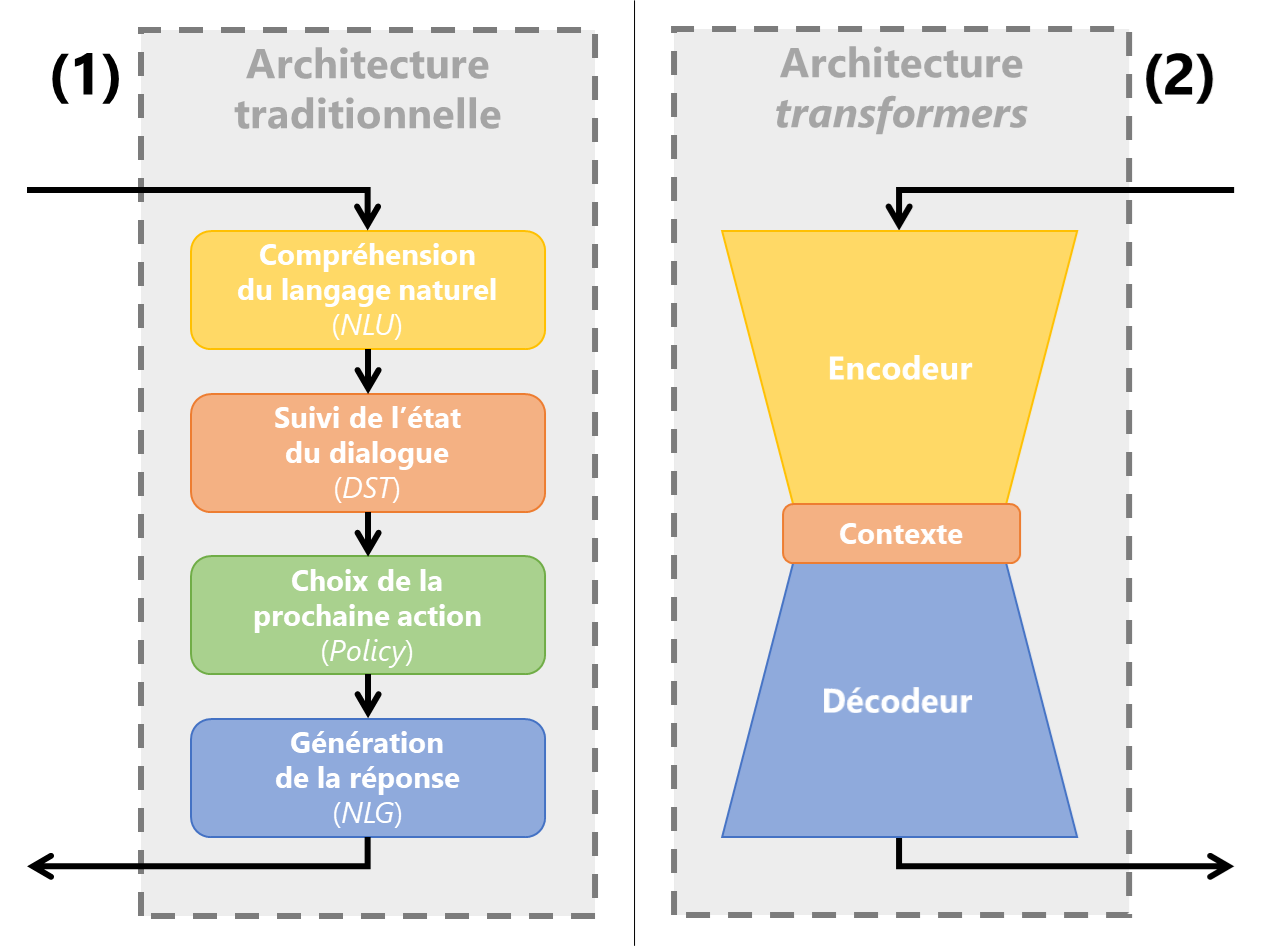
\includegraphics[width=0.90\textwidth]{figures/annexe-chatbots-architectures}
			\caption{
				Schéma illustrant les deux approches principales de conception d'un assistant conversationnel :
				\textbf{(1)} représente les \textbf{approches \textit{task-oriented}} à l'aide d'une architecture manipulant des états de dialogue ;
				\textbf{(2)} représente les \textbf{approches \textit{chat-oriented}} à l'aide d'une architecture à base de \textit{transformers}, encodant et décodant numériquement le dialogue et son contexte.
			}
			\label{figure:B.2-ANNEXE-CHATBOT-APPROCHES}
		\end{figure}
		
		
		%%%
		%%% Approches \textit{task-oriented}.
		%%%
		
		% Description.
		Les \textbf{approches orientées par tâche} (\textit{task-oriented}) considèrent la conversation comme une succession d'étapes menant à une action précise : le système est donc conçu pour collecter les informations nécessaires et interagir avec un moteur d'actions dans le but d'accomplir un objectif.
		Ainsi, ces approches reposent généralement sur une modélisation fine du parcours utilisateur permettant de s'assurer de l'exécution pas à pas des actions intermédiaires de la tâche demandée.
		
		% Achitecture.
		La \textsc{Figure~\ref{figure:B.2-ANNEXE-CHATBOT-APPROCHES}} \textbf{(1)} représente l'architecture traditionnellement utilisée pour concevoir ce type d'assistants.
		Cette architecture est composée de quatre éléments principaux :
		\begin{itemize}
			% NLU.
			\item le \textcolor{colorCarrotOrange}{\texttt{NLU}} (\textit{Natural Language Understanding}) :
				ce composant utilise un ensemble de concepts pour interpréter le dialogue de manière symbolique.
				Cette modélisation du dialogue, généralement implémentée à l'aide de méthodes supervisées, repose sur des détections de \textit{domaines} (\textit{thématique générale traitée}), des détections de \textit{sentiments} (\textit{positif, négatif ou neutre}), des détections d'\textit{intentions} (\textit{action exprimée par l'utilisateur, manifesté par le verbe d'action}), ou encore des extractions d'\textit{entités} (\textit{ensemble de mentions textuelles pertinentes}) (voir \cite{adamopoulou-moussiades:2020:overview-chatbot-technology}) ;
			% DST.
			\item le \textcolor{colorDarkPastelGreen}{\texttt{DST}} (\textit{Dialogue State Tracking}) :
				ce composant utilise les concepts détectés précédemment par le \texttt{NLU} (\textit{domaine}, \textit{sentiment}, \textit{intentions}, \textit{entités}) pour déterminer l'objectif de l'utilisateur et mettre à jour l'état de la conversation ;
			% PL.
			\item la \textcolor{colorDarkPastelGreen}{\texttt{PL}} (\textit{Policy Learning}) : 
				ce composant choisit la prochaine action de l'assistant sur la base de l'état du dialogue déterminé par le \texttt{DST}.
				Ce choix peut être réalisé par un ensemble de règles, mais aussi grâce à un apprentissage supervisé ou à un apprentissage par renforcement (voir \cite{brabra-etal:2022:dialogue-management-conversational}) ;
			% NLG.
			\item la \textcolor{colorSilverLakeBlue}{\texttt{NLG}} (\textit{Natural Language Generation}) :
				ce dernier composant affiche une réponse à l'utilisateur qui soit en adéquation avec l'action choisie par la \texttt{PL}.
				Cette réponse peut être paramétrée à l'avance ou être générée à la volée.
		\end{itemize}
		
		
		% Avantages et inconvénients.
		Cette approche est rudimentaire mais efficace, et elle est utilisée pour concevoir une grande partie des assistants dans un cadre industriel :
		\begin{itemize}
			\item[\faThumbsUp] 
			% Implémentation facile.
				Les différents composants de l'architecture sont simples à implémenter et à maintenir
				(\textit{ces différentes briques sont indépendantes et ont des fonctionnalités bien précises}) ;
				% Paramétrage facile.
				de nouvelles règles de dialogues peuvent facilement être ajoutées dans le système
				(\textit{du moins si les processus de ces tâches sont bien documentés}) ;
				% Mise sous contrôle.
				il est facile de contrôler le comportement de l'assistant
				(\textit{il suffit de fixer certaines règles de dialogue dans le \texttt{DST} et dans la \texttt{PL}}) ;
				% Infrastructure légère.
				cette architecture simple consomme peu de ressources de la machine (\textit{les modèles de détections et la gestion des règles peuvent tourner sur \texttt{CPU}}).
			\item[\faThumbsDown] Cependant :
				% Couts initiaux.
				les coûts initiaux peuvent être importants (\textit{notamment en ce qui concerne la collecte et la modélisation des données d'apprentissage, ou encore la définition des parcours de dialogue pour des tâches non documentées}) ;
				% Modélisation sensible aux erreurs.
				la compréhension du langage est limitée (\textit{certaines erreurs ou ambiguïtés de langage rendent les détections du \texttt{NLU} non adaptées ou non performantes}) ;
				% Peu flexible.
				le dialogue est très peu flexible, et le périmètre de l'assistant est réduit à ce qui a été modélisé (\textit{le dialogue peut être bloqué ou rejeté si aucune règle n'est prévue pour la demande de l'utilisateur ou pour l'état courant}).
		\end{itemize}
		
		\newpage
		
		% Exemple fictif.
		\begin{leftBarExamples}
			Pour illustrer nos propos, analysons la demande fictive suivante :
			\begin{quote}
				\begin{center}
					\textguillemets{\textit{
						Je veux réserver un billet de train pour Strasbourg.
					}}
				\end{center}
			\end{quote}
			\begin{itemize}
				\item le \texttt{NLU} pourrait détecter le domaine "\texttt{voyage}", l'intention "\texttt{réservation}" et les entités "$\textit{billet de train}_{\texttt{(produit)}}$" et "$\textit{Strasbourg}_{\texttt{(gare\_destination)}}$" ;
				\item le \texttt{DST} pourrait établir l'objectif de réserver un train, mais que les informations \texttt{(date\_départ)} et \texttt{(gare\_départ)} sont manquantes ;
				\item la \texttt{PL} pourrait décider de demander d'abord le complément d'information sur la gare de départ (\textit{et demandera la prochaine information plus tard}) ;
				\item la \texttt{NLG} pourrait sortir une phrase de réponse prédéfinie pour demander le complément d'information à l'utilisateur.
			\end{itemize}
		\end{leftBarExamples}
			
		% Exemples réels
		\begin{leftBarExamples}
			Nous pouvons citer les projets ou outils suivants :
			\begin{itemize}
				\item \texttt{RASA} (\cite{bocklisch-etal:2017:rasa-open-source}) et \texttt{WATSON} (\cite{hoyt-etal:2016:ibm-watson-analytics}) sont deux moteurs de dialogue basés sur une approche symbolique et manipulant des intentions et des entités ;
				\item \texttt{Assistant Virtuel SNCF} (\cite{sncf:2018:agent-virtuel-sncf}), \texttt{Google Assistant} (\cite{google:2016:google-assistant-your}) et \texttt{Alexa} (\cite{alexa-internet:2018:keyword-research-competitor}) sont des assistants connus pour être orientés par tâches, les deux derniers pouvant même être paramétrables par l'utilisateur final pour ses usages en domotiques ;
				\item \cite{yan-etal:2017:building-taskoriented-dialogue} décrivent un projet de conception d'un assistant conversationnel pour du commerce en ligne.
			\end{itemize}
		\end{leftBarExamples}
		
		\newpage
		
		%%%
		%%% Approches \textit{chat-oriented}.
		%%%
		
			\todo[inline]{
				A REDIGER: \textit{chat-oriented}\\
				Axée dialogue \\
				Quelques exemples \\
				Architecture transformers: encodeur/décodeur, tout est numérique \\
				Pas de contrôle (hallucination) \\
				Grande flexibilité
			}
			
			% Description.
			Les \textbf{approches \textit{chat-oriented}}
			
			% Avantages et inconvénients.
			\begin{itemize}
				\item[\faThumbsUp] Les avantages : ;
				\item[\faThumbsDown] Les inconvénients : .
			\end{itemize}
			
			% Exemples.
			\begin{leftBarExamples}
				TODO
			\end{leftBarExamples}
			
			%%% DEFINITIONS
			% Un \textit{chatbot} \textguillemets{\textit{chat-oriented}} se concentre davantage sur les interactions avec l'utilisateur dans le but d'\textbf{engager la conversation}.
			% Son objectif principale est de rendre le dialogue agréable.
			% Son périmètre de connaissance n'est en général pas restreint pour pouvoir facilement engager la conversation sur n'importe quel sujet.
			
			% ARCHITECTURE
			% \texttt{GPT} (\cite{openai:2023:chatgpt})
			% ou \texttt{LLAMA2} (\cite{touvron-etal:2023:llama-open-foundation}).
			% \cite{uszkoreit:2017:transformer-novel-neural}  \\ % architecture transformers
			% \cite{ni-etal:2022:recent-advances-deep}  \\ % avancer en deep learning
			% \cite{openai:2023:chatgpt}  \\ % exemple
			% \cite{touvron-etal:2023:llama-open-foundation}  \\ % exemple
			% \cite{kaddour-etal:2023:challenges-applications-large} % plusieurs challenges
			
			%%% FONCTIONNALITES
			% Offrir du divertissement (\textit{raconter une histoire ou une blague, organiser un jeu narratif, ...}) ;
			% Proposer une assistance générale (\textit{donner une définition, demander une explication, ...}) ;
			% Simplement discuter (\textit{mimer les interactions sociales}).
		
		%%%
		%%% Approches hybrides.
		%%%
		
			\todo[inline]{
				A REDIGER: \textit{hybride}\\
				LLM instruct \\
				DST entraînée \\
				NLG décodeur
			}
			
			% Définitions.
			Les \textbf{approches hybrides}
			
			% Exemples.
			\begin{leftBarExamples}
				TODO
			\end{leftBarExamples}
	
	
	%%%%%--------------------------------------------------------------------
	%%%%% Annexe B.3: Dilemme de conception : entre flexibilité et contrôle.
	%%%%%--------------------------------------------------------------------
	\section{Dilemme de conception : entre flexibilité et contrôle}
	\label{annex:B.3-ANNEXE-CHATBOTS-DILEMME}
		
		\todo[inline]{A REDIGER: niveau d'automatisation}
		% \cite{sheridan-verplank:1978:human-computer-control} repris par \cite{parasuraman-etal:2000:model-types-levels} \\ % 10 niveaux de contrôles